\documentclass{article} % For LaTeX2e
\usepackage{iclr2026_conference,times}
\usepackage{graphicx} % 添加这一行来支持 \includegraphics
\input{math_commands.tex}
% \usepackage{hyperref}
% \usepackage[hidelinks]{hyperref}
\definecolor{iccvblue}{rgb}{0.21,0.49,0.74}

\usepackage[pagebackref,breaklinks,colorlinks,allcolors=iccvblue]{hyperref}
\usepackage{url}
\usepackage{amsmath}
\usepackage{amssymb}
\usepackage{booktabs}
\usepackage{multirow}
\usepackage[table,xcdraw]{xcolor}
\usepackage{tcolorbox}
\definecolor{best}{HTML}{C8E6C9}
\definecolor{best2}{HTML}{BBDEFB}
\definecolor{grey}{HTML}{e0e0e0}
\usepackage{algorithm}
\usepackage{algorithmic}
\usepackage{pifont}
\usepackage{cuted} 
\usepackage{newfloat}
\usepackage{listings}
\usepackage{soul}
\sethlcolor{grey!90} % 设置高亮颜色为浅灰
\usepackage{wrapfig}
\usepackage{caption}  % for \captionof
\usepackage{tocloft}
\usepackage{etoc}
\usepackage{enumitem}
\title{\textbf{From Editor to Estimator}: Diffusion Tran\\sformer-based Dense Geometry Prediction}
\author{1}
\newcommand{\fix}{\marginpar{FIX}}
\newcommand{\new}{\marginpar{NEW}}
\newcommand{\cxx}[1]{\textcolor{red}{Comments from cxx: #1}}
\newcommand{\wjy}[1]{Respond from wjy: #1 \textcolor{blue}{Have improved!}}
\begin{document}

\maketitle
\vspace{-2em}
\begin{figure}[h]
   \centering
   \vspace{-1em}
   \includegraphics[width = 0.99\linewidth]{first2.pdf} 
   \vspace{-1em}
   \caption{We present \textbf{FE2E}, a DiT-based foundation model for monocular dense geometry prediction. With limited training data, FE2E achieves tremendous performance improvements in zero-shot depth and normal estimation. Bar length indicates the average ranking across all metrics from multiple datasets, where lower values are better. \ding{72} represents the amount of training data used.}
   \label{fig:first}
   \vspace{-1em}
\end{figure}

\begin{abstract}
  \vspace{-1em}
   Leveraging visual priors from pre-trained text-to-image generative models has shown success in dense prediction. However, dense prediction is inherently an image-to-image task, suggesting that image editing models, rather than generators, may be a more suitable foundation for fine-tuning.
   Motivated by this, we conduct a systematic analysis of the fine-tuning behaviors of both editors and generators for dense geometry estimation. Our findings show that editing models possess inherent structural understanding, enabling them to converge more stably by ``refining" existing features, and ultimately achieve higher performance than their generative counterparts.
   Based on these insights, we introduce \textbf{FE2E}, a framework that pioneeringly adapts an advanced editing model based on Diffusion Transformer (DiT) architecture for dense geometry prediction. Specifically, to tailor the editor for this deterministic task, we reformulate the editor's original flow matching loss into the ``consistent velocity" training objective. And we use logarithmic quantization to resolve the precision conflict between the editor's native BFloat16 format and the high precision demand our tasks.
   Additionally, we leverage the DiT's built-in global attention mechanism to design a cost-free joint estimation strategy, which allows the model to output both depth and normals in a single forward pass, and enables the supervisory signals mutually enhance one another. Without scaling up the training data, FE2E achieves unprecedented performance improvements in both zero-shot monocular depth and normal estimation across multiple datasets, including over 35\% performance gains in the ETH3D dataset and outperforms the DepthAnything series, which is trained on 100$\times$ data.
\end{abstract}

\section{Introduction}
\begin{figure}[!t]  
  \centering
  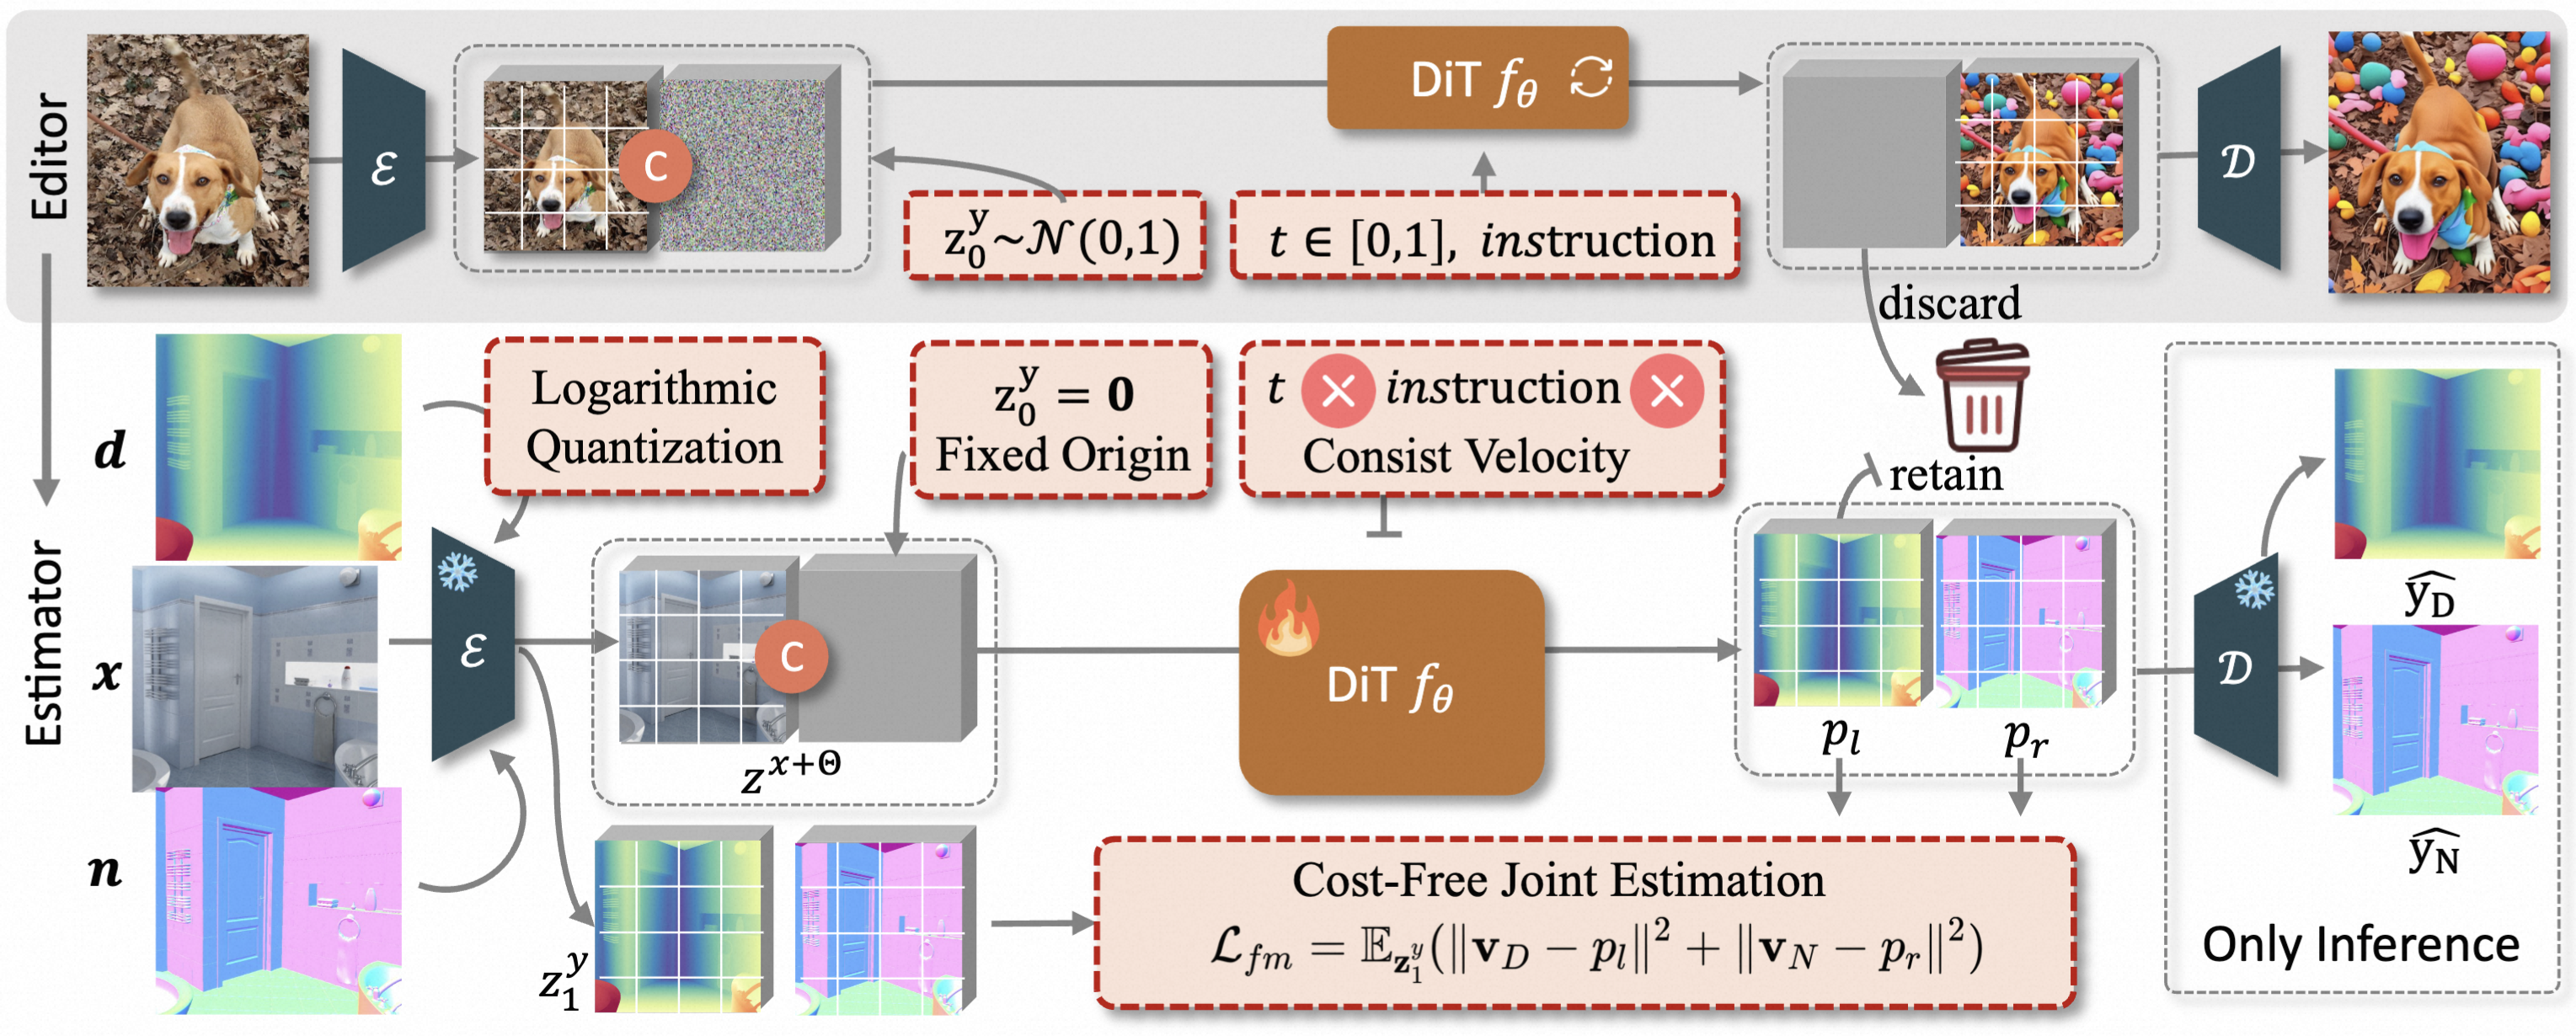
\includegraphics[width=\textwidth]{pipeline.pdf}
  \caption{\textbf{FE2E Adaptation Pipeline.} The \colorbox{grey}{grey background} shows the original editor's workflow, while the other details FE2E: \ding{172} A pre-trained VAE encodes the logarithmically quantized depth $\mathbf{d}$, input image $\mathbf{x}$, and normals $\mathbf{n}$ into latent space. \ding{173} The DiT $f_\theta$ learns a constant velocity $\mathbf{v}$ from a fixed origin $\mathbf{z}^y_0$ to the target latent $\mathbf{z}^y_1$, independent of $t$ or instructions. \ding{174} By repurposing the discarded output region, FE2E jointly predicts depth and normals without extra computation. Training loss is computed in the latent space, with final predictions decoded by VAE only at inference.}
  \label{fig:pipeline}
  \vspace*{-1em}
\end{figure}
Dense geometry prediction tasks, such as depth/normal estimation, are crucial for a wide range of applications such as augmented reality~\citep{ar}, and 3D reconstruction~\citep{3dgs}. 
Estimating pixel-level geometric attributes from a single image is an ill-posed problem and can only be solved with the help of prior knowledge, such as typical object shapes and sizes, occlusion patterns, etc. %
Based on this observation, recent works ingeniously leverage the priors from pre-trained text-to-image (T2I) generators, typically Stable Diffusion~\citep{sd}, for zero-shot dense prediction~\citep{marigold}, yielding impressive results with limited training data.

However, these generative models are initially designed for T2I generation and lack the ability to capture the geometric cues from the absent image inputs. In contrast, image editing models have recently risen to be a universal framework to solve more diversified image-to-image (I2I) tasks, such as semantic segmentation and depth estimation~\citep{qwenimage}. We argue that, these editing models not only align with the dense estimation paradigm but also possess a deep understanding of input images while maintaining the generative advantages, offer a more suitable foundation for dense geometry prediction.

Motivated by this intuition, we systematically analyze the fine-tuning dynamics of the 
image editing models versus its generative counterparts. Our analysis reveals a crucial finding: editing model's features have an inherent alignment with geometric structures, and subsequent fine-tuning only requires to ``refine" and ``focus" this ability for dense estimation tasks. In contrast, while generative models can gradually acquire this capabilities from scratch, this process leads to substantial feature reshaping and cannot fundamentally bridge this gap (Sec.~\ref{sec:analysis}). Therefore, in this paper, we explore this \textbf{From Editor to Estimator} option and propose \textbf{FE2E} (Fig.~\ref{fig:pipeline}), a diffusion transformer (DiT) model built upon current SoTA editor Step1X-Edit~\citep{step}, along with a fine-tuning protocol to adapt it for dense geometry prediction tasks.

Clearly, although image editing and dense prediction are both I2I tasks, a direct transfer of editing formulation is still suboptimal due to the task differences. 
First, compare to editing, the dense geometry prediction is more deterministic, as only one unique ground-truth (GT) exists. Our analysis of Step1X-Edit reveals that its training objectives—predicting \textit{instantaneous velocity}\footnote{velocity denotes the direction and speed of transformation that ``change input to output", see Sec.~\ref{sec:preliminaries}}—is only tailored for indeterminate tasks and can introduce errors in dense prediction. Based on this observation, we reformulate the training objective as a \textit{consistent velocity}$^1$ and set a fixed starting point for stable training. 
Second, image editing models like Step1X-Edit are typically trained with BF16 precision, which is sufficient for RGB outputs, whereas dense geometry prediction tasks like depth estimation demand much higher numerical precision. This discrepancy does not occur in previous adopted foundation models like Stable Diffusion v1.5/v2, which offer FP32 checkpoints. To overcome this limitation and improve computational efficiency, we analyze the GT quantization strategies and ultimately adopt logarithmic quantization to alleviate precision-related artifacts.

After adapting the editor, we now focus on its role as an estimator. In this paper, we select two primary geometry prediction tasks: zero-shot depth estimation and normal estimation, to validate FE2E's effectiveness. Depth and normal both contribute to a unified geometric representation of 3D shapes, and joint estimation can reasonably utilize their potential connections. Unlike prior methods that introduce extra modules like cross-attention or switchers, we observe that the global attention mechanism of DiT can be repurposed to produce multiple outputs from a single input. Consequently, FE2E jointly estimates depth and normals within a single forward pass at virtually no additional computational cost. This design allows the supervisory signals from both tasks to interact, mutually enhancing the overall performance.

Extensive experiments demonstrate that our model achieves tremendous zero-shot performance improvements compared to previous same kind state-of-the-art (SoTA) models (\textbf{35\%} AbsRel improvement on the ETH3D dataset). Furthermore, even when using only \textbf{0.2\%} of the training data, FE2E outperforms the data-driven models like DepthAnything v1/v2. Our contribution can be summarized as follows:
\begin{itemize}[leftmargin=*,nosep]
  \item We systematically analyze the fine-tuning dynamics of image editors and generators, revealing that editing models are more suitable for dense geometry prediction. Accordingly, we introduce FE2E, a novel framework that, for the first time, successfully adapts a pre-trained image editing model for this task.
  \item We identify and address the challenges that arise from this paradigm shift: 1)Reformulate the training objective to align with dense prediction deterministic nature; 2)Adopt a logarithmic quantization to resolve the precision conflict.
 \item We design a cost-free joint estimation strategy that allows mutual information exchange between different prediction tasks. Based on our enhancement, FE2E achieves tremendous performance gains on both zero-shot monocular depth and surface normal estimation.
\end{itemize}

\vspace{-1em}
\section{Related Work}
\vspace{-0.5em}
\textbf{Image Generative and Editing models}
In the field of image generation, Stable Diffusion series~\citep{sd} and FLUX series~\citep{flux} models have basically become the community standard. They both trained with massive datasets and demonstrate extremely high generation quality. Concurrently, the field of image editing is still evolving rapidly. Recent advancements include Step1X-Edit~\citep{step}, a model fine-tuned from FLUX, which demonstrates superior instruction-following and image understanding capabilities; The multi-modal Qwen-Image~\citep{qwenimage} Editor combines with LLM, attempting to expand the editor into a unified computer vision framework. We conduct a more detail review in the appendix Sec~\ref{supp:related}.
\newline\textbf{Dense Geometry Estimation,} encompassing tasks like depth and normal estimation, is a cornerstone of 3D computer vision. Early research predominantly focused on supervised learning paradigms, where models were trained and evaluated on specific datasets~\citep{eigen,eigen2}. A significant shift occurred with MiDaS~\citep{midas}, which pioneered cross-dataset generalization for dense estimation. This line of work was extended by models like DPT~\citep{dpt} and Omnidata~\citep{omini}, which further improved zero-shot performance. More recently, the field has witnessed the rise of data-driven models such as Depth Anything series~\citep{dam1,dam2} and the Metric3D series~\citep{metric3d}, which leverage massive datasets to train powerful, general-purpose geometric estimators.
\newline
\textbf{Generative Models for Dense Estimation.}
In parallel to this trend of scaling up data, an alternative approach emerged by leveraging the rich priors of pre-trained generative models. Works like Marigold~\citep{marigold} and GeoWizard~\citep{geowizard} showed that fine-tuning diffusion models on limited data could yield remarkable performance, effectively harnessing the models' learned world knowledge. This paradigm was further refined by GenPercept~\citep{genprecept}, StableNormal~\citep{stablen}, Diffusion-E2E-FT~\citep{e2eft}, Lotus~\citep{lotus}, and Jasmine~\citep{jasmine}. These studies identified and addressed the limitations of standard diffusion formulations, developing the single-step denoising architecture to boost performance. In this paper, we also build FE2E with limited data, posit that the I2I editing models are inherently better than the T2I models, like Stable Diffusion~\citep{sd} for dense estimation.

\section{Methods}
\vspace{-0.5em}
For clarity, we term the direct adaptation of the original editing/generative formulation as \textit{``DirectAdapt''} (Sec~\ref{sec:preliminaries}), and Table~\ref{tab:ablation} shows that \textit{DirectAdapt} fails to achieve satisfactory performance. To address this, we introduce two key improvements on training objective (Sec~\ref{sec:consistent}) and GT quantization(Sec~\ref{sec:quantization}). They can benefit both editing and generative models, and these \textit{improved} models are better for analyzed our core motivation (Sec~\ref{sec:analysis}), as they isolate the error from training data and the denoising process. We finally introduce joint training on the editing-based model to obtain \textbf{FE2E}.
\begin{figure}[!t]  
  \centering
  \vspace{-2em}
  \includegraphics[width=\textwidth]{flux.pdf}
  \vspace{-2em}
  \caption{
    \textbf{Comparison between the Generative and Editing foundation models.} We analyze the feature evolution at both the initial (Epoch 1) and final (Epoch 30) stages of fine-tuning, resulting into 4 groups. Each group present: the DiT features at input end (Block1), middle layers (Block20), output end (Block35), and the final estimated depth. Visual implementation detailed in Sec~\ref{supp:gen}.
}
  \label{fig:flux}
  \vspace{-1.5em}
\end{figure}
\vspace{-1em}
\subsection{Fine-tuning Dynamic Analysis of Editor and Estimator}
\label{sec:analysis}
\begin{wrapfigure}{r}{0.5\textwidth}
  \vspace{-1em}
  \centering
  \includegraphics[width = \linewidth]{flux2.pdf}
  \vspace{-2em}
  \caption{\textbf{Quantitative comparison of the training loss} between Generative and Editing foundation models. The main plot details the \textit{convergence} loss from epoch 5 to 30, while the inset displays the steep \textit{initial} loss reduction during the first 10 epochs, which occurs on a different scale.}
  \vspace{-2em}
  \label{fig:flux2}
\end{wrapfigure}
We chose Step1X-Edit as our foundation model, which is the SoTA editor when this work launched, and FE2E can also generalize to other DiT-based editing models. Step1X-Edit is finetuned from the generative model FLUX, and they share an identical DiT architecture. To justify our choice, we additionally trained a FLUX-based model (implementation details in Sec~\ref{supp:gen}) and performed a systematic analysis that reveals \textbf{3} key advantages of using an editing-based model over its generative predecessor for dense estimation tasks.

First, \hl{the editing model possesses a superior inductive bias for image-to-image dense estimation tasks, providing a much stronger starting point for finetuning.} This is qualitatively evident in Fig.~\ref{fig:flux} (a1 \textit{v.s.} a2), in early stage and blocks, the editor’s internal features already align with the input image's geometric structures, while the generative ones are abstract and unstructured.  The loss difference in Fig.~\ref{fig:flux2} \ding{72} shows the same conclusion.

Second, this above difference directly impacts the learning dynamics: as illustrated in Fig.~\ref{fig:flux2}, the editor achieves a more stable convergence, in contrast to the oscillations seen in the generative ones. This difference can be further explained in Fig.~\ref{fig:flux}, \hl{the fine-tuning process significantly reshapes the characteristics of generative models, while the editor's features are more like a ``refinement" and ``focusing"}. After 30 epochs fine-tuning, the generated model learned highly structured and semantic features (a4, b4, c4) from chaotic states (a2, b2, c2), achieving a qualitative leap. Whereas the editing ones makes the well-structured features (a1, b1, c1) clearer and task oriented (a3, b3, c3), with its features being incrementally honed rather than fundamentally altered.

Third, \hl{the ``structured learning" and ``characteristics reshaping" mentioned above  unable to cover the shortage of the generative model.} As shown in Fig.~\ref{fig:flux2} (epochs 20-30, especially $\blacklozenge$), the generative model's training loss meet a bottleneck around 0.08, while the editing ones can reduce to 0.073. The Table~\ref{tab:ablation} (ID7 vs. ID8) further indicate that this bottleneck persists at test time, resulting in a significant performance gap.

In summary, both feature evolution, training dynamics, and the performance gap consistently show that the editing models offer a more \textbf{stable, effective, and potential} foundation for dense geometry estimation.
\subsection{From Editor To Estimator}
\label{sec:preliminaries}

As shown in Fig.~\ref{fig:pipeline}, we pose monocular dense estimation as a image editing task and use the \textbf{Flow Matching} Loss for supervision. 

Initially, we take the input image $\mathbf{x} \in \mathbb{R}^{H \times W \times 3}$ as the editing source and the geometric annotation $\mathbf{y} \in \mathbb{R}^{H \times W \times 3}$ as the expected editing results. First, the auto-encoder, which consists an encoder $\mathcal{E}(\cdot)$ and a decoder $\mathcal{D}(\cdot)$, is used to encode the input image $\mathbf{x}$ into a latent representation $\mathbf{z}^x = \mathcal{E}(\mathbf{x})\in \mathbb{R}^{h \times w \times c}$. 
Then, the editing process is modeled as a flow path from a noise vector $\mathbf{z}^y_0 \sim \mathcal{N}(0, \mathbf{I})$ to the target latent representation $\mathbf{z}^y_1 = \mathcal{E}(\mathbf{y})$. The trajectory is defined as:
\begin{equation}
\label{eq:rectified_flow}
    \mathbf{z}^y_t = t \mathbf{z}^y_1 + (1-t) \mathbf{z}^y_0, \quad t \in [0, 1].
\end{equation}
The DiT backbone, denoted as $f_\theta$, is trained to predict the \textbf{velocity vector} of this flow, which is simply $\mathbf{v} = \frac{d\mathbf{z}^y_t}{dt} = \mathbf{z}^y_1 - \mathbf{z}^y_0$. The model is optimized by minimizing the flow matching loss~\citep{flowmatch}:
\begin{equation}
    \label{eq:loss_original}
        \mathcal{L} = \mathbb{E}_{t,\mathbf{z}^y_1, \mathbf{z}^y_0} \| \mathbf{v} - f_\theta(\mathbf{z}^x, \mathbf{z}^y, t) \|^2.
\end{equation}
In the inference stage, we predict the editing target $\hat{\mathbf{z}}^y_1$ by solving the following ordinary differential equation:
\begin{equation}
\label{eq:ode}
\hat{\mathbf{z}}^y_1 = \mathbf{z}^y_0 + \int_0^1 f_\theta(\mathbf{z}^x,\mathbf{z}^y, t) dt ,
\end{equation}%这里要改一下,加上c
and the final dense geometry predictions are given by $\hat{\mathbf{y}} = \mathcal{D}(\hat{\mathbf{z}}^y_1)$. The more details of the flow matching process are provided in Sec~\ref{supp:flow}.


\subsection{Consistent Velocity Flow Matching with Deterministic Departure}
\label{sec:consistent}
\begin{wrapfigure}{r}{0.5\textwidth}
    \vspace{-6mm}
    \centering
    \includegraphics[width = 1.0\linewidth]{meanflow.pdf}
    \caption{\textbf{Left}: GT velocity field for network training. The gray dots represent different Gaussian noise (top) or \textbf{zero} starting points (bottom), the red dots represent data samples. \textbf{Right}: Instantaneous velocity $v$ determines the tangent direction and create errors in the cumulative path (top); The constant speed path is a straight line.
    }%删去后缺乏为啥这样
    \vspace{-6mm}
    \label{fig:meanflow}
\end{wrapfigure}

Since the Flow Matching introduction, it has seen widespread adoption in modern generative and editing modeling. As shown in Fig.~\ref{fig:meanflow}, previous work MeanFlow~\citep{meanflow} has identified that, because the model learns the  velocity over all possible flow paths in Eq~\ref{eq:rectified_flow}, the global instantaneous velocity field becomes inherently non-linear and typically induces a curved trajectory. 

During inference, as shown in Fig.~\ref{fig:meanflow} (b), the ideal integration path in Eq.~\ref{eq:ode} is approximated by a discrete numerical solver. While the resulting approximation error is negligible for non-deterministic tasks like image editing or generation, our experiments show it becomes significant for high-precision tasks such as dense estimation.

An intuitive idea is to find a straight integration path, which means the velocity direction always remains the same. In this paper, we further require the velocity magnitude be consistent so that the velocity is completely independent of $t$, redefine the loss as:
\begin{equation}
	\label{eq:loss_consistent}
			\mathcal{L} = \mathbb{E}_{\mathbf{z}^y_1,\mathbf{z}^y_0} \| \mathbf{v} - f_\theta(\mathbf{z}^x,\mathbf{z}^y) \|^2.
\end{equation}
Additionally, one key characteristic of generative/editing models is their stochastic nature, which is essential for producing diverse outputs. For deterministic dense prediction tasks, however, this stochasticity is not only unnecessary but also introduces undesirable variance into the training objective, complicating the optimization of $f_\theta$. Therefore, we simplify the objective by reducing it from a stochastic expectation over all possible $\mathbf{z}^y_0$ to a deterministic formulation with a fixed $\mathbf{z}^y_0 = \mathbf{0}$. This further refine the loss as:
\begin{equation}
  \label{eq:loss_simplified}
      \mathcal{L} =  \mathbb{E}_{\mathbf{z}^y_1} \|\mathbf{v} - f_\theta(\mathbf{z}^x) \|^2,
\end{equation}
and the inference process can be simplified as:
\begin{equation}
  \label{eq:inference_simplified}
      \mathbf{z}^y_1 = \mathbf{z}^y_0 + \int_0^1 f_\theta(\mathbf{z}^x) dt = \mathbf{0} + (1-0)f_\theta(\mathbf{z}^x) = f_\theta(\mathbf{z}^x).
\end{equation}
Overall, as shown in Fig.~\ref{fig:meanflow} (c) and (d), our refined flow matching not only eliminates the errors introduced by discretized curved trajectory and random starting points, but also significantly reduces inference time, achieving simultaneous improvements in both performance and efficiency.


\subsection{Logarithmic Annotation Quantization}
\label{sec:quantization}
\input{tb0.tex}
Nowadays, modern generative/editing models are almost exclusively trained with BF16 precision. This is not only because BF16 precision saved the training cost, but also for their typical outputs, RGB images, this precision is entirely sufficient. Specifically, a normalized BF16 value is represented as:
$$
V = (-1)^{S} \times 2^{(E - 127)} \times (1.F)_{2},
$$
where S is the sign (1 bit), E is the exponent (8 bits), and F is the fraction (7 bits). Due to the required input data range of [-1,1] for the Step1x-Edit VAE (a common practice for generative and editing models), the worst-case precision occurs at $\pm$[0.5, 1.0], which is $2^{126-127} \times 2^{-7}=1/{256}$ and perfectly satisfies the RGB range of 0-255.  

Uncritically finetuning these models with FP32, as done in Marigold or Lotus, not only increases training/inference costs, but also leads to suboptimal inheritance of the baseline model's priors, and restricts the capabilities of BF16-only models like Step1X-Edit. Therefore, finetuning with BF16 is necessary.

However, as shown in Fig.~\ref{fig:quantization} (a,b), when meet the depth annotations in Virtual KITTI dataset, the valid depth range is 0-80m. \textbf{Directly} regularizing to [-1,1] requires a reduction of 40 times and the accuracy of 1/256 is reflected in the original depth with a significant error of 40/256$\approx$0.16m. This errors results in an AbsRel of 1.6 at 0.1m (Table \ref{tab:errbf16} (a)) and make the finetune process unfeasible. Previous works have employed a \textbf{inverse} quantization scheme, which means converting the reciprocal of the depth, or disparity, to BF16 precision (Fig.~\ref{fig:quantization} (c, d)). As shown in Table~\ref{tab:errbf16} (b), despite offering extremely high precision at close ranges, this scheme becomes entirely unusable at greater distances, even makes 39m and 78m correspond to the same value. The principles and calculation are details in Sec~\ref{supp:quant}.

After numerous attempts and explorations, we finally use the \textbf{logarithmic} depth quantization to achieve good precision at both near and far ranges (Table~\ref{tab:errbf16}(c)) while reducing training and inference costs. Specifically, we first logarithmic depth with ${D}_{log}=ln({D}_{GT}+1e-6)$, then follow and refined the Marigold's depth normalization strategy, defining the supervision label $\mathbf{y}_D$ as:
\begin{equation}
    \label{eq:log_quantization}
		\mathbf{y}_D = \left\langle \left( \frac{({D}_{log}-{D}_{log,2})}{({D}_{log,98}-{D}_{log,2})} - 0.5 \right) \times 2 \right\rangle,
\end{equation}
where ${D}_{log,i}$ corresponds to the $i\%$ percentiles of ${D}_{log}$, and $\langle\cdot\rangle$ is the BF16 precision truncation.

\subsection{Cost-Free Joint Estimation }
\label{sec:joint}
There are inherent connections between depth and normal, as both contribute to a unified geometric representation of 3D shapes. Normals describe surface variations and undulations, while depth outlines the spatial arrangement that guides the orientation of the normals. Thus, previous work like GeoWizard~\citep{geowizard} attempted to control the SD model with a geometry switcher, but this approach doubled the training cost.

In contrast, as shown in Fig.~\ref{fig:pipeline}, Step1X-Edit and other DiT-based editing works have found that, the DiT architecture can effectively guided image generation by horizontally concatenating the noise and condition latents, that is, the input is formulated as $z^{x+\Theta}=\text{concat}(z^x, z^\Theta) \in \mathbb{R}^{h \times 2w \times c}$. However, after processing by the DiT, although the model's output has the same shape as the input, $f_\theta(z^{x+\Theta}) = [p_l, p_r] \in \mathbb{R}^{h \times 2w \times c}$, supervision is only applied to the region corresponding to the original noise, i.e., $\mathcal{L} = \|\mathbf{v} - p_r\|^2$, where $p_l, p_r \in \mathbb{R}^{h \times w \times c}$.

It is worth noting that DiT architecture possesses the global attention across the $(h, 2w)$ dimension, which naturally allows for mutual information exchange and high consistency between $p_l$ and $p_r$. Based on this observation, without introducing any additional training or inference costs, we additionally incorporate another task's supervision on $p_l$ during finetuning, modifying the flow matching loss to:
\begin{equation}
  \label{eq:loss_joint}
      \mathcal{L}_{fm} =  \mathbb{E}_{\mathbf{z}^{y}_1}( \|\mathbf{v}_D - p_l \|^2 +  \|\mathbf{v}_N - p_r \|^2).
\end{equation}
\begin{figure}[!t]
\vspace{-0.5em}
  \includegraphics[width = 1.0\linewidth]{visu.pdf}
  \vspace{-2em}
  \caption{\textbf{Quantitative comparison on zero-shot depth and normal estimation.} The 1st row shows the input, the 2nd, 3rd rows are previous SoTA methods results, and the 4th row is ours prediction. White arrows highlight the regions we significantly improve. Zoom in for better view.
  }
  \label{fig:visual}
  \vspace{-1em}
\end{figure}
\vspace{-1em}
\section{Experiments}
\subsection{Training Loss and Implementation Details} 
To further enhance the DiT's representational power, we also introduce an auxiliary dispersion loss that encourages features from different samples to spread out in the hidden space. Following Diffuse-and-Disperse~\citep{disperse}, we apply this loss to the output of the 9th block:
\begin{equation}
\label{eq:loss_disperse}
\mathcal{L}_{\text {disp}}=\log \mathbb{E}_{i, j}\left[\exp(-\|\eta_{i}-\eta_{j}\|_{2}^{2}/ \tau) \right],
\end{equation}
where $\eta_{i,j}$ are the output features for the $i$-th and $j$-th samples in a batch, respectively, and temperature $\tau=1$. Finally, the training loss is defined as: $\mathcal{L}_{train} = \mathcal{L}_{fm} + \lambda \mathcal{L}_{\text {disp}}, \lambda=0.5$. The choices of $\lambda$, $\tau$, and block all follow the optimal hyper-parameters identified in the experiments from Diffuse-and-Disperse.

We build FE2E upon the Step1X-Edit v1.0 framework~\citep{step}. During finetuning, all parameters except for the DiT module are frozen, and the language control input is left blank. The process employs LoRA~\citep{lora} with rank $=64$ and scale factor $\alpha=32$. We trained for 30 epochs using the AdamW optimizer~\citep{adamw} with an initial learning rate of $1 \times 10^{-4}$. With gradient checkpoint enabled, the model can be trained on a single RTX 4090 GPU, but to accelerate experimentation, training was conducted on NVIDIA H20 GPUs, completing in approximately 1.5 days. The training dataset, evaluation dataset, and evaluation metrics are detailed in Sec~\ref{supp:traindata}, \ref{supp:evadata}, \ref{supp:metric}, respectively.
\vspace{-1em}
\subsection{Quantitative Evaluation}
\begin{table}[!ht]
  \scriptsize
  \vspace{-1em}
  \caption{\textbf{Quantitative comparison on zero-shot affine-invariant depth estimation} between FE2E and SoTA methods. The \colorbox{best}{best} and \colorbox{best2}{second best} performances are highlighted. $^\star$ denotes the method relies on pre-trained Stable Diffusion.}
  \vspace{-3mm}
  \label{tab:depth}
  \resizebox{\textwidth}{!}{
  \setlength{\tabcolsep}{2pt}
  \setlength{\extrarowheight}{1pt}
  \begin{tabular}{l|c|cc|cc|cc|cc|cc|c}
  \toprule
  \multirow{2}{*}{Method}& Training & \multicolumn{2}{c|}{NYUv2 (Indoor)} & \multicolumn{2}{c|}{KITTI (Outdoor)} & \multicolumn{2}{c|}{ETH3D (Various)} & \multicolumn{2}{c|}{ScanNet (Indoor)} & \multicolumn{2}{c|}{DIODE (Various)} & Avg \\
  % &
  & Data$\downarrow$ & AbsRel$\downarrow$ & $\delta$1$\uparrow$ &  AbsRel$\downarrow$ & $\delta$1$\uparrow$ & AbsRel$\downarrow$ & $\delta$1$\uparrow$ &  AbsRel$\downarrow$ & $\delta$1$\uparrow$ & AbsRel$\downarrow$ & $\delta$1$\uparrow$ & Rank$\downarrow$ \\
  \midrule
  
MiDaS 
& 2M & 11.1 & 88.5  & 23.6 & 63.0  & 18.4 & 75.2  & 12.1 & 84.6  & 33.2 & 71.5  & 10.6 \\

GeoWizard 
% & 280K & 5.2 & 96.6  & 9.7& 92.1  & 6.4 & 96.1  & 6.1 & 95.3  & 29.7 & 79.2 & 5.4 \\
& 280K & 5.6 & 96.3  & 14.4& 82.0  & 6.6 & 95.8  & 6.4 & 95.0  & 33.5 & 72.3 & 8.4 \\

GenPercept 
% & 74K & 5.6 & 96.0  & 9.9 & 90.4  & 6.2 & 95.8  & - & -  & 35.7 & 75.6  & 8.2 \\
& 74K & 5.6 & 96.0  &13.0 & 84.2  & 7.0 & 95.6  & 6.2 & 96.1  & 35.7 & 75.6  & 7.8 \\

Marigold$_\text{v1.1}$$^{\star}$
& 74K & 5.8 & 96.1  & 11.0 & 88.8 & 7.0& 95.5  & 6.6 & 95.3  & 30.4 & 77.3 & 7.6\\

Marigold$^{\star}$ 
& 74K & 5.5 & 96.4  & 9.9 & 91.6  & 6.5 & 95.9 & 6.4 & 95.2  & 30.8 & 77.3  & 6.3 \\

DepthAnything V2
& 62.6M & 4.5 & \cellcolor{best2}97.9  & \cellcolor{best2}7.4 & 94.6  & 13.1 & 86.5  & -& -  & 26.5 & 73.4 & 5.4 \\

Lotus-G$^{\star}$ 
& \cellcolor{best}{59K} & 5.4 & 96.8  & 8.5 & 92.2  & \cellcolor{best2}5.9 & \cellcolor{best2}97.0  & 5.9 & 95.7  & \cellcolor{best2}22.9 & 72.9 & 4.7 \\

Diffusion-E2E-FT$^{\star}$ 
& 74K & 5.4 & 96.5  & 9.6 & 92.1  & 6.4 & 95.9  & 5.8 & 96.5  & 30.3 & \cellcolor{best2}77.6 & 4.6 \\

Lotus-D$^{\star}$
& \cellcolor{best}{59K} & 5.1 & 97.2 & 8.1 & 93.1  & 6.1 & \cellcolor{best2}97.0 & 5.5 & 96.5 & \cellcolor{best2}22.8 & 73.8  & \cellcolor{best2}3.7 \\

DepthAnything 
& 62.6M & \cellcolor{best2}4.3 & \cellcolor{best}98.1  & 7.6 & \cellcolor{best2}94.7  & 12.7 & 88.2  & \cellcolor{best}4.3 & \cellcolor{best}98.1 & 26.0 & 75.9 & 3.5\\

\textcolor{black}{\textbf{FE2E}}
& \cellcolor{best2}\textcolor{black}{\textbf{71K}} & \textcolor{black}{\cellcolor{best}\textbf{4.1}} & \textcolor{black}{97.7}  & \textcolor{black}{\cellcolor{best}\textbf{6.6}} & \textcolor{black}{\cellcolor{best}\textbf{96.0}}  & \textcolor{black}{\cellcolor{best}\textbf{3.8}} & \textcolor{black}{\cellcolor{best}\textbf{98.7}}  & \textcolor{black}{\cellcolor{best2}\textbf{4.4}} & \textcolor{black}{\cellcolor{best2}\textbf{97.5}}  & \textcolor{black}{\cellcolor{best}\textbf{22.8}} & \textcolor{black}{\cellcolor{best}\textbf{81.2}}  & \textcolor{black}{\cellcolor{best}\textbf{1.4}} \\
  \bottomrule
  \end{tabular}
  }
  \vspace{-1.5em}
\end{table}

\paragraph{Zeroshot Depth Estimation Comparison}
As presented in Table~\ref{tab:depth}, FE2E significantly outperforms recent SoTA methods across five challenging benchmarks. Notably, on the ETH3D and KITTI datasets, \hl{it reduces the AbsRel error by \textbf{35\%} and \textbf{10\%} respectively, compared to the 2nd-best method.} Remarkably, despite being trained on only \textbf{0.071M} images, FE2E's average rank surpasses that of the DepthAnything series, which was trained on a massive \textbf{62.6M} image dataset. This highlights the effectiveness of our strategy: inheriting the editing model priors rather than simply scaling up training data. Furthermore, qualitative comparisons in Fig.~\ref{fig:first} and \ref{fig:visual} demonstrate that \hl{FE2E produces superior results in challenging lighting conditions (extreme-light, low-light, etc.) and better preserves distant details,} which 
intuitively reveal the core advantages that contribute to FE2E's superior performance. We provide further comparisons with concurrent unified works in Sec~\ref{supp:exp}.

\begin{table}[!ht]
  \caption{\textbf{Quantitative comparison on zero-shot surface normal estimation} between FE2E and SoTA methods. $^\ddag$refers the Marigold normal model as detailed in this. }
  \vspace{-3mm}
  \label{tab:normal}
  \scriptsize
  % \small
  \centering
  
  \resizebox{\textwidth}{!}{
  \setlength{\tabcolsep}{3pt}
  \setlength{\extrarowheight}{1pt}
  \begin{tabular}{l|c|cc|cc|cc|cc|c}
  
  \toprule
  \multirow{2}{*}{Method}
  % &\multirow{2}{*}{Venue}
  & Training
  & \multicolumn{2}{c|}{NYUv2 (Indoor)} & \multicolumn{2}{c|}{ScanNet (Indoor)} 
  & \multicolumn{2}{c|}{iBims-1 (Indoor)} & \multicolumn{2}{c|}{Sintel (Outdoor)}
  
  & \textcolor{black}{Avg.} \\
   % &
   &Data$\downarrow$
   & MeanErr$\downarrow$ & $11.25^\circ$$\uparrow$  
   & MeanErr$\downarrow$ & $11.25^\circ$$\uparrow$ 
   & MeanErr$\downarrow$ & $11.25^\circ$$\uparrow$ 
   & MeanErr$\downarrow$ & $11.25^\circ$$\uparrow$ 
  
   &    \textcolor{black}{Rank}           \\
  \midrule
  


Marigold$^{\ddag\star}$
% &CVPR 2024 
&74K& 20.9 & 50.5 & 21.3 & 45.6 & 18.5 &64.7& -  & -    & 9.5\\
GeoWizard$^{\star}$
% &ECCV 2024
&280K& 18.9 & 50.7 & 17.4 & 53.8 & 19.3 & 63.0 & 40.3 & 12.3 & 8.9          \\

GenPercept$^{\star}$
% &ICLR 2025
&74K& 18.2 & 56.3 & 17.7 & 58.3 & 18.2 & 64.0 & 37.6 & 16.2 & 7.4            \\

StableNormal$^{\star}$
% &SIGGRAPH 2024 
&250K& 18.6 & 53.5 & 17.1 & 57.4 & 18.2 & 65.0 & 36.7 & 14.1& 7.2  \\

Lotus-G$^\ast$ 
% &ICLR 2025
&\cellcolor{best}59K&  16.5&  59.4&  15.1&  63.9&  17.2&  66.2&  33.6&  21.0& 5.2 \\

DSINE 
% &CVPR 2024
&160K& 16.4 & 59.6  & 16.2 & 61.0 & 17.1 & 67.4 &34.9 & 21.5 & 4.6   \\

Lotus-D$^\star$
% &ICLR 2025
&\cellcolor{best}59K& \cellcolor{best2}16.2 & 59.8  & 14.7& 64.0  & 17.1 &66.4&\cellcolor{best2}32.3&\cellcolor{best}22.4 & 3.0  \\

Diffusion-E2E-FT$^{\star}$
% &WACV 2025
& 74K& 16.5 & \cellcolor{best2}60.4& {14.7} & \cellcolor{best2}66.1& \cellcolor{best2}16.1 &\cellcolor{best2}69.7&33.5 & \cellcolor{best2}{22.3} & 2.6  \\


Marigold$_{v1.1}$ $^\ast$ 
% &-
&77K & \cellcolor{best} {16.1}& \cellcolor{best}60.5& \cellcolor{best2}14.5&  \cellcolor{best2}66.1&  16.3& 68.5& -& -& \cellcolor{best2}2.0  \\

\textbf{FE2E}$^\ast$
% &- 
&\cellcolor{best2}\textbf{71K}&  \cellcolor{best2}\textbf{16.2}&  59.6& \cellcolor{best}\textbf{13.8}&\cellcolor{best}  \textbf{67.2}&  \cellcolor{best}\textbf{15.1}&\cellcolor{best}  \textbf{70.6}&  \cellcolor{best}\textbf{31.2}& \cellcolor{best2}\textbf{ 22.3}& \textcolor{black}{\cellcolor{best}\textbf{1.6}}   \\
  
  \bottomrule
  \end{tabular}
  }
\vspace{-1.5em}
\end{table}

\paragraph{Zeroshot Normal Estimation Comparison}
As presented in Table~\ref{tab:normal}, FE2E also achieves SoTA performance on the zero-shot normal estimation task, outperforming the methods in recent 2 years across four benchmarks. This quantitative superiority stems from its ability to handle complex geometries. As illustrated in Fig.~\ref{fig:first}, \ref{fig:visual}, \hl{FE2E excels at reconstructing intricate details such as surface folds and small objects}, which are often challenging for other models.
\subsection{Ablation Study}
\label{sec:ablation}
\textbf{Effect of Foundation Model}
FE2E is based on a new foundation model, which may raise concerns regarding the source of the performance improvement. In Table~\ref{tab:ablation}, comparison between ID2 and ID9 shows that using Step1X-Edit without improvement ,performance decreases by 47\% and 44\% on the ETH3D and KITTI datasets, respectively (AbsRel, the same below), which strongly indicates the genuine performance gains reason.

\textbf{Effect of Editing Priors}
We trained the FLUX-based model under both \textit{DirectAdapt} and \textit{Improved} settings, corresponding to ID1 and ID8 in Table~\ref{tab:ablation}. Compared with their counterparts (ID2 and ID7), the editing-based models consistently outperform the generative models, regardless of equipping our proposed improvements. These results, together with the findings in Sec~\ref{sec:analysis}, highlight the effectiveness of leveraging editing model priors for dense prediction tasks.

\textbf{Effect of Improved Flow Matching}
Adopting the consistent velocity training objective effectively eliminates accumulated inference errors from the original paradigm, leading to notable performance gains of 7\% on KITTI and 10\% on ETH3D (ID2 \textit{v.s.} ID3). Introducing a fixed starting point further eases optimization and brings additional improvements(ID3 \textit{v.s.} ID4).

\textbf{Effect of Data Quantization}
Supervision leads to substantial performance gains, with ID7 and ID5 achieving 19\% and 13\% improvements on the KITTI and ETH3D datasets, respectively. Notably, inverse quantization (ID6) generally outperforms direct quantization, typically due to there are more valid pixels nearby.

\begin{wrapfigure}{r}{0.6\textwidth}
  \centering
  \vspace{-1.5em}
  \includegraphics[width = 1.0\linewidth]{LR.pdf}
  \vspace{-1em}
  \caption{Qualitative comparison on the Joint Estimation. The `w/o Joint Estimation' shows 2 models' results.}
  \label{fig:joint}
  \vspace{-1em}
\end{wrapfigure}

\textbf{Effect of Joint Estimation and Disperse Loss}
Results from ID7 and ID9 demonstrate that joint prediction further enhances model performance. This synergistic effect is more clearly illustrated in Fig.~\ref{fig:joint}, where joint training yields notable improvements in challenging scenarios such as flat butterfly structures, and distant buildings. Additionally, we conducted ablation studies on the disperse loss, which is not a core component of our method. The performance gains observed in ID4 and ID5 confirm that this loss is also effective for dense geometric estimation tasks.
\begin{table}[!ht]
  \scriptsize
  \centering
  \vspace{-1.5em}
  \caption{ \label{tab:ablation}\textbf{Ablation studies} on the step-by-step design of our adaptation protocol for fitting pre-trained generative/editing models into dense geometric prediction. Here we show the results in zero-shot depth estimation. The meaning of abbreviation (CV: Consistent Variance; FS: Fixed Start; DL: Disperse Loss; JE: Joint Estimation; Quant: Quantization, sub-items same with Table~\ref{tab:errbf16}).}
  \resizebox{\textwidth}{!}{
     \setlength{\tabcolsep}{5pt}
     \begin{tabular}{c|c|c|c|c|c|c|c|cc|cc}
  \toprule
       \multirow{2}{*}{ID}& \multirow{2}{*}{Note} &\multirow{2}{*}{Foundation}& \multirow{2}{*}{CV}&\multirow{2}{*}{FS}& \multirow{2}{*}{DL}&\multirow{2}{*}{JE}& \multirow{2}{*}{Quant}&\multicolumn{2}{c|}{{KITTI}} & \multicolumn{2}{c}{{ETH3D}}  \\
      & & & & & && & AbsRel$\downarrow$ & $\delta1\uparrow$ & AbsRel$\downarrow$ & $\delta1\uparrow$ \\
      \midrule
      1  &\textit{DirectAdapt}& Flux & & & &  & Direct & 9.7&91.2&6.0&96.0 \\
      2  &\textit{DirectAdapt}& Step1X-Edit  &  &  & &  & Direct & 9.5&91.4&5.6&96.2 \\
      3  & & Step1X-Edit  &  \ding{51} & & & & Direct  & 8.8&93.2&5.0&97.2 \\
      4  & & Step1X-Edit  &  \ding{51} &\ding{51} & & & Direct  & 8.6&94.0&4.8&97.3\\
       5  & & Step1X-Edit  &  \ding{51} &\ding{51} &\ding{51}& & Direct  & 8.4&94.4&4.5&97.6\\
      6  & & Step1X-Edit  &  \ding{51} & \ding{51}& \ding{51}& & Inverse & 6.9&95.1&4.6&98.2 \\
      7 &\textit{Improved}&Step1X-Edit  &  \ding{51} & \ding{51}&\ding{51}& & Logarithmic & \cellcolor{best2}6.8&\cellcolor{best2}95.6&\cellcolor{best2}3.9&\cellcolor{best2}98.6 \\
      8  &\textit{Improved}& Flux &  \ding{51} & \ding{51} & \ding{51} & & Logarithmic & 7.1&94.9&4.5&97.8 \\
      9  &\textbf{FE2E}&\textbf{Step1X-Edit } &  \ding{51} & \ding{51} & \ding{51} & \ding{51} &\textbf{Logarithmic}  & \cellcolor{best}\textbf{6.6}&\cellcolor{best}\textbf{96.0}&\cellcolor{best}\textbf{3.8}&\cellcolor{best}\textbf{98.7} \\
  \bottomrule
     \end{tabular}
     }
     \vspace{-0.8cm}
  \end{table}
\section{Conclusion}
\vspace{-0.5em}
In this paper, our systematic analysis shows that editors provide a more stable and effective foundation than their generative counterparts. Based on this, we introduced \textbf{FE2E}, a novel framework that successfully adapts a pre-trained editing model for dense geometry prediction. To bridge the gap between these tasks, we proposed a consistent velocity training objective for stable convergence and logarithmic quantization to resolve precision conflicts. We also designed a cost-free joint estimation strategy, enabling mutual enhancement within a single forward pass. FE2E achieves SoTA performance and validates the \textbf{`From Editor to Estimator'} paradigm, showcasing that harnessing the inherent ability of editing models is a effective and data-efficient approach for dense prediction.

\appendix
\section*{Appendix}
In this appendix, we provide more implementation details, experiments, analysis, and discussions for a comprehensive evaluation and understanding of FE2E. Detailed contents are listed as follows:

\setlength{\cftbeforesecskip}{0.5em}
\cftsetindents{section}{0em}{1.8em}
\cftsetindents{subsection}{1em}{2.5em}
\etoctoccontentsline{part}{Appendix}
{
  \etocsettocstyle{}{}
  \localtableofcontents
}

% \hypersetup{linkbordercolor=red,linkcolor=red}

\section{Experiment Settings}

\subsection{Training Datasets} 
\label{supp:traindata}
We train our model for joint depth and normal estimation on a mixture of two synthetic datasets: Hypersim~\citep{hypersim} and Virtual KITTI~\citep{vkitti}. 
From \textbf{Hypersim}, a photorealistic indoor dataset, we use its official training split after filtering out samples with over 1\% invalid pixels, resulting in approximately 51k images at a 1024$\times$768 resolution. 
From \textbf{Virtual KITTI}, a synthetic street view dataset, we utilize four driving scenarios, totaling around 20k samples at a 1216$\times$352 resolution with a maximum depth of 80m. 
Following Marigold, each training batch is constructed by sampling from Hypersim and Virtual KITTI with probabilities of 90\% and 10\%, respectively. 

\subsection{Evaluation Datasets}
\label{supp:evadata}
We evaluate our model on two tasks: \textbf{Zero-shot Affine-Invariant Depth Estimation.} We evaluate on five standard benchmarks: NYUv2~\citep{nyuv2}, ScanNet~\citep{scannet}, KITTI~\citep{kitti}, ETH3D~\citep{eth3d}, and DIODE~\citep{diode}. Following standard practice, we report the Absolute Relative error (AbsRel) and $\delta_1$ accuracy. \textbf{Surface Normal Prediction.} We evaluate on NYUv2, ScanNet, iBims-1~\citep{ibims}, and Sintel~\citep{sintel} benchmarks. The evaluation metrics are the mean angular error (MeanErr) and the percentage of pixels with an angular error below $11.25^{\circ}$. 

\subsection{Evaluation Metrics}
\label{supp:metric}
For zero-shot depth estimation, similar to \citep{marigold}, we employ the following  evaluation metrics:
\begin{itemize}
  \item AbsRel:  $\ \frac{1}{|{M}_{vl}|} \sum_{d \in {M}_{vl}}\left|d-d_{gt}\right| / d_{gt}$;
  \item ${a}_{1}$: percentage of $d$ such that $\max(\frac{d}{d_{gt}},\frac{d_{gt}}{d}) < 1.25$ ;
\end{itemize}
where $d_{gt}$ and $d$ denote the GT and estimated pixel depth, ${M}_{vl}$ is the valid mask (mask rules are consistent with \citep{lotus}). 

For zero-shot normal estimation, we use the following evaluation metrics:
\begin{itemize}
\item $
\text{MeanErr} = \frac{1}{|{M}_{vl}|} \sum_{\mathbf{n} \in {M}_{vl}} \frac{180}{\pi} \arccos(\text{clamp}(\mathbf{n} \cdot \mathbf{n}_{gt}, -1, 1))
$

\item \textbf{$11.25^{\circ}$}: The percentage of $\mathbf{n}$ where the angular error is less than $11.25^{\circ}$;
\end{itemize}
where $\mathbf{n}_{gt}$ and $\mathbf{n}$ denote the GT and estimated normal vector.

\section{Implementation Details of Generative-base Models}
\label{supp:gen}
Step1X-Edit is fine-tuned from the generative model FLUX, and both share an almost identical DiT architecture. To further reduce confounding factors, we follow the Step1X-Edit protocol and replace the original FLUX input with a horizontally concatenated noise and RGB image. All hyperparameters, including LoRA settings, optimizer, and training data, are kept exactly the same as those used for FE2E in depth estimation.

FLUX consists of 38 block layers, each producing outputs of consistent dimensions. After rearrangement, the feature map has the shape $B \times 192 \times H/8 \times W/8$, where B is batchsize, H and W are height and width of the input image. Typically, the output from the final block is projected to 16 channels and passed to the VAE for reconstruction to $B \times 3 \times H \times W$. For visualization, we chose 1, 20, and 35 blocks, operate on the $B \times 192 \times H/8 \times W/8$ feature map, normalize it to $B \times 1 \times H/8 \times W/8$ using the L2 norm, upsample it to $B \times 1 \times H \times W$, and finally visualize it using the Rainbow colormap. The visualization of depth and normals follows the approach of Lotus.

Since our experimental comparisons are conducted using the \textit{improved} model, only a single ``denoising" step is performed during inference. Consequently, the output from the VAE decoder directly represents the depth map (the $B \times 3 \times H \times W$ output mentioned before was averaged to obtain a 1-channel depth map), which makes it easier to visualize meaningful features.

\section{Quantization Error Calculation Details}
\label{supp:quant}

The following calculations are based on the effective depth range of 0-80m from the Virtual KITTI dataset. The normalization scheme consistently maps an input domain $X$ to the VAE's mandatory input range of [-1, 1] using the standard min-max scaling formula: $V = 2 \times \frac{X - X_{min}}{X_{max} - X_{min}} - 1$. While other mapping schemes from [0m, 80m] to [-1, 1] may exist, they are not explored in this work. All calculations use the worst-case precision of BF16 over the [-1, 1] interval, which corresponds to a single quantization step of $\Delta V \approx 1/256$.

\subsection{Direct Quantization}
In this scheme, the depth value $D$ is linearly mapped to the [-1, 1] interval. The depth range is $[D_{min}, D_{max}] = [0\text{m}, 80\text{m}]$.
The mapping function is $V = 2 \times \frac{D - 0}{80 - 0} - 1 = \frac{D}{40} - 1$.
A quantization step of $\Delta V = 1/256$ in the normalized space corresponds to an error $\Delta D$ in the real-world depth space. This error is constant across the entire depth range:
$$\Delta D = 40 \times \Delta V = 40 \times \frac{1}{256} \approx 0.15625$$

{At 80m}:
Error $\approx {16cm}$.
AbsRel = $\frac{0.16\text{m}}{80\text{m}} = {0.002}$.

{At 0.1m}:
Error $\approx {16cm}$.
AbsRel = $\frac{0.16\text{m}}{0.1\text{m}} = {1.600}$.

This method yields an unacceptably large relative error at close distances.

\subsection{Inverse Quantization}
This scheme quantizes the reciprocal of depth, i.e., disparity $P = 1/D$. We consider an effective depth range of $[0.1\text{m}, 80\text{m}]$ to avoid division by zero.
The corresponding disparity range is $[P_{min}, P_{max}] = [1/80, 1/0.1] = [0.0125, 10]$.
The disparity $P$ is linearly mapped to [-1, 1]. The quantization step in disparity, $\Delta P$, is constant:
$$\Delta P = (P_{max} - P_{min}) \times \frac{\Delta V}{2} = (10 - 0.0125) \times \frac{1/256}{2} \approx 0.0195.$$
The relationship between depth error $\Delta D$ and disparity error $\Delta P$ is given by $\Delta D \approx |\frac{d(1/P)}{dP}| \Delta P = \frac{1}{P^2}\Delta P = D^2 \Delta P$.

{At 80m}:
Error = $(80\text{m})^2 \times 0.0195 = 6400 \times 0.0195 \approx 124.8\text{m} \approx {125m}$.
AbsRel = $\frac{125\text{m}}{80\text{m}} \approx {1.563}$.

{At 0.1m}:
Error = $(0.1\text{m})^2 \times 0.0195 = 0.01 \times 0.0195 = 0.000195\text{m} \approx {0.2mm}$.
AbsRel = $\frac{0.0002\text{m}}{0.1\text{m}} = {0.002}$.
        
As mentioned in the main text, the disparities for 39m and 78m are $1/39 \approx 0.0256$ and $1/78 \approx 0.0128$, respectively. Their difference is $\approx 0.0128$, which is smaller than the disparity quantization step $\Delta P \approx 0.0195$, making them indistinguishable after quantization. This scheme fails completely at large distances.

\subsection{Logarithmic Quantization}
This scheme quantizes the logarithmic depth, $D_{log} = \ln(D)$. We again consider the depth range $[0.1\text{m}, 80\text{m}]$.
The corresponding log-depth range is $[\ln(0.1), \ln(80)] \approx [-2.30, 4.38]$.
The log-depth $D_{log}$ is linearly mapped to [-1, 1]. The quantization step in log-depth, $\Delta D_{log}$, is constant:
$$\Delta D_{log} = (\ln(80) - \ln(0.1)) \times \frac{\Delta V}{2} = (4.38 - (-2.30)) \times \frac{1/256}{2} \approx 0.013.$$
The relationship between depth error $\Delta D$ and log-depth error $\Delta D_{log}$ is given by $\Delta D \approx |\frac{d(e^{D_{log}})}{dD_{log}}| \Delta D_{log} = e^{D_{log}} \Delta D_{log} = D \cdot \Delta D_{log}$.
This implies that the absolute relative error, AbsRel = $\Delta D / D$, is approximately constant and equal to $\Delta D_{log} \approx 0.013$.

{At 80m}:
AbsRel $\approx {0.013}$.
Error = $80\text{m} \times 0.013 = 1.04\text{m}$.

{At 0.1m}:
AbsRel $\approx {0.013}$.
Error = $0.1\text{m} \times 0.013 = 0.0013\text{m} = {1.3mm}$.
        
This method maintains a reasonable and nearly constant relative error across both near and far ranges, making it a well-balanced and effective solution. The percentile-based normalization used in the main text is a more robust implementation of this fundamental principle.

\section{Preliminaries of Flow Matching}
\label{supp:flow}

Flow Matching \citep{flowmatch} is a highly effective framework for training Continuous Normalizing Flows (CNFs). The core idea is to smoothly transform a simple prior distribution $p_0$ (e.g., the standard Gaussian distribution $\mathcal{N}(0, \mathbf{I})$) into a complex target data distribution $p_1$ over a continuous time variable $t \in [0, 1]$.

This transformation process can be described by an Ordinary Differential Equation (ODE), where the velocity at any time $t$ and point $\mathbf{z}$ is defined by a vector field $v_t(\mathbf{z})$. However, estimating this marginal vector field $v_t(\mathbf{z})$ directly from data samples is challenging. The Flow Matching framework elegantly bypasses this issue by regressing a much simpler and easier-to-compute conditional vector field $u_t(\mathbf{z} | \mathbf{z}_0, \mathbf{z}_1)$ instead.

Specifically, we first sample a pair of points, $(\mathbf{z}_0, \mathbf{z}_1)$, from the prior distribution $p_0$ and the target distribution $p_1$, respectively. We then define a simple path $\mathbf{z}_t$ from $\mathbf{z}_0$ to $\mathbf{z}_1$ and its corresponding conditional vector field $u_t = \frac{d\mathbf{z}_t}{dt}$. It has been proven that if a neural network $f_\theta(\mathbf{z}, t)$ is trained to approximate this simple conditional vector field $u_t$, then in expectation over all sample pairs $(\mathbf{z}_0, \mathbf{z}_1)$ and time $t$, the network $f_\theta$ will converge to the complex marginal vector field $v_t$ that we truly wish to learn.

\paragraph{Rectified Flow}
\citep{rectified_flow} presents a particularly simple and powerful instance of Flow Matching. It defines the path between $\mathbf{z}_0$ and $\mathbf{z}_1$ as a straight line:
$$
    \mathbf{z}_t = t \mathbf{z}_1 + (1-t) \mathbf{z}_0, \quad t \in [0, 1].
$$
The derivative of this path is trivial, yielding a constant velocity vector that is independent of both time and space:
$$
    \mathbf{v} = \frac{d\mathbf{z}_t}{dt} = \mathbf{z}_1 - \mathbf{z}_0.
$$
Consequently, the training objective (loss function) becomes exceedingly simple: aligning the neural network's prediction with this constant velocity vector $\mathbf{v}$:
$$
    \mathcal{L} = \mathbb{E}_{t, \mathbf{z}_1, \mathbf{z}_0} \| (\mathbf{z}_1 - \mathbf{z}_0) - f_\theta(\mathbf{z}_t, t) \|^2.
$$

\paragraph{Application in \textit{DirectAdapt}}
In this paper, we adapt this framework for a conditional image editing task. Our goal is not to learn an unconditional generative model, but rather a flow from noise $\mathbf{z}^y_0$ to the target geometry latent $\mathbf{z}^y_1$, guided by the input image $\mathbf{x}$ (encoded as $\mathbf{z}^x$). Therefore, our velocity prediction model $f_\theta$ must take $\mathbf{z}^x$ as an additional condition. As shown in Eq.~\ref{eq:loss_original} in the main text, our loss function is:
$$
    \mathcal{L} = \mathbb{E}_{t,\mathbf{z}^y_1, \mathbf{z}^y_0} \| (\mathbf{z}^y_1 - \mathbf{z}^y_0) - f_\theta(t, \mathbf{z}^x) \|^2.
$$
During inference, we generate the target latent $\hat{\mathbf{z}}^y_1$ by solving the following ODE, with $\mathbf{z}^x$ serving as the guiding condition:
$$
\frac{d\hat{\mathbf{z}}^y_t}{dt} = f_\theta(t, \mathbf{z}^x), \quad \text{with initial value } \hat{\mathbf{z}}^y_0 \sim \mathcal{N}(0, \mathbf{I}).
$$
By integrating from $t=0$ to $t=1$ using a numerical ODE solver (e.g., Euler method), we can obtain the final prediction $\hat{\mathbf{z}}^y_1$.

\section{Reviews of Related Generative and Editing Models}
\label{supp:related}
The fields of image generation and image editing have always been complementary, and they have undergone several paradigm shifts. The first major breakthrough was the Generative Adversarial Network (GAN)~\citep{gan}, which introduced a novel adversarial training process. Then, key advancements in this era include architectural refinements like DCGAN~\citep{dcgan}, the development of conditional and text-to-image GANs such as the StackGAN series~\citep{zhang2017stackgan, zhang2018stackgan++}, AttnGAN~\citep{xu2018attngan}, and Cross-Modal Contrastive Learning based models~\citep{zhang2021cross}. The StyleGAN series~\citep{StyleGAN1, StyleGAN2, StyleGAN3} marked a high point for GANs, achieving unprecedented photorealistic high-resolution image synthesis and offering fine-grained control over visual attributes through a disentangled latent space, which became a cornerstone for many subsequent editing techniques.

More recently, the field has transitioned to Denoising Diffusion Models~\citep{ho2020denoising}, which have become the state-of-the-art for their superior image quality and textual coherence. A series of influential diffusion-based methods were introduced, including GLIDE~\citep{nichol2021glide}, DALL$\cdot$E~\citep{dalle} and its successor DALL$\cdot$E~2~\citep{unclip}, Imagen~\citep{imagen}, and PIXART-$\alpha$~\citep{pixart}. The open-source Stable Diffusion (SD)~\citep{sd} model, trained on the large-scale LAION-5B dataset~\citep{schuhmann2022laion}, further democratized high-quality image generation and quickly became a community standard. The recent FLUX series~\citep{flux} employ a novel Diffusion Transformer design that challenges the prevalence of U-Nets and achieves remarkable generation speed and quality.

Building on these powerful generative foundations, the domain of image editing (generalized editing) has also advanced rapidly. Early diffusion-based methods like SDEdit~\citep{meng2021sdedit} demonstrated that real images could be edited by adding noise and then denoising with a new text prompt. A significant leap was made with instruction-guided editing, pioneered by InstructPix2Pix~\citep{instructpix2pix}, which enabled edits based on natural language commands. The field has since diversified with numerous innovative approaches. For instance, DragGAN~\citep{pan2023draggan} introduced a novel point-based interaction, allowing users to ``drag" pixels to precisely deform object shapes. OmniControl~\citep{omnicontrol} further enhances controllability by creating a unified framework that accepts diverse spatial guidance signals for both synthesis and editing. This trend towards more powerful and versatile models is also reflected in large-scale systems like UniWorld~\citep{uniworld}, which uses a unified transformer for multi-modal understanding and generation, Step1X-Edit~\citep{step}, fine-tuned from the FLUX architecture for superior instruction following, and multi-modal editors like Qwen-Image~\citep{qwenimage}, which leverage Large Language Models (LLMs) to build more comprehensive visual editing frameworks.

\section{Addition Experiments Results}
\label{supp:exp}
\begin{table}[!ht]
  \scriptsize
     \centering
     \caption{Quantitative comparison on zero-shot affine-invariant depth estimation between FE2E and concurrent unified model. }
     \label{tab:exp}
  \resizebox{\textwidth}{!}{
  \setlength{\tabcolsep}{3pt}
  \setlength{\extrarowheight}{1pt}
     \begin{tabular}{l|cc|cc|cc|cc|cc|c}
  \toprule
  \multirow{2}{*}{Method} 
  % &\multirow{2}{*}{Venue}
   & \multicolumn{2}{c|}{NYUv2 (Indoor)} & \multicolumn{2}{c|}{KITTI (Outdoor)} & \multicolumn{2}{c|}{ETH3D (Various)} & \multicolumn{2}{c|}{ScanNet (Indoor)} & \multicolumn{2}{c|}{DIODE (Various)} & Avg \\
  % &
  & AbsRel$\downarrow$ & $\delta$1$\uparrow$ &  AbsRel$\downarrow$ & $\delta$1$\uparrow$ & AbsRel$\downarrow$ & $\delta$1$\uparrow$ &  AbsRel$\downarrow$ & $\delta$1$\uparrow$ & AbsRel$\downarrow$ & $\delta$1$\uparrow$ & Rank$\downarrow$ \\
  \midrule
  
  Qwen-Image
  % &ICLR 2025
  & 5.5 & 96.7 & 7.8 & 95.1  & 6.6 & 96.2 &4.7 & 97.4 & \cellcolor{best}19.7 & \cellcolor{best}83.2  &2.6 \\
  
  DINOv3
  % &ICLR 2025
   & \cellcolor{best2}4.3 & \cellcolor{best}98.0 & \cellcolor{best2}7.3 &\cellcolor{best} 96.7  & \cellcolor{best2}5.4 &\cellcolor{best2} 97.5 &\cellcolor{best2}4.4 &\cellcolor{best} 98.1 & 25.6 & \cellcolor{best2}82.2  &\cellcolor{best2}1.8\\
  
  \textcolor{black}{\textbf{FE2E}}
  % & -- 
   & \textcolor{black}{\cellcolor{best}\textbf{4.1}} & \textcolor{black}{\cellcolor{best2}\textbf{97.7}}  & \textcolor{black}{\cellcolor{best}\textbf{6.6}} & \textcolor{black}{\cellcolor{best2}\textbf{96.0}}  & \textcolor{black}{\cellcolor{best}\textbf{3.8}} & \textcolor{black}{\cellcolor{best}\textbf{98.7}}  & \textcolor{black}{\cellcolor{best}\textbf{4.4}} & \textcolor{black}{\cellcolor{best2}\textbf{97.5}}  & \textcolor{black}{\cellcolor{best2}\textbf{22.8}} & \textcolor{black}{81.2}  & \textcolor{black}{\cellcolor{best}\textbf{1.6}} \\
  
  
  \bottomrule
  \end{tabular}
     }
  \end{table}

\paragraph{Comparison with Concurrent Unified Model}
The field of dense geometry estimation is advancing rapidly, with the task of depth estimation particularly fast. Recently, several concurrent works have been explored to unify the visual tasks, which also include depth estimation benchmarks. As shown in Table~\ref{tab:exp}, our method consistently achieves the top average ranking, even though they are trained with extremely huge data compared to FE2E (e.g., Qwen Image utilizes billions of samples, and DINO v3 is trained on 1.7 billion images).

\paragraph{Additional Qualitative Comparison}
Fig.~\ref{fig:append1} present a qualitative comparison between FE2E and other methods. The results demonstrate that our approach produces more refined and accurate depth predictions, particularly in structurally complex regions that may not be fully captured by quantitative metrics. Furthermore, as illustrated in Fig.~\ref{fig:append2}, Lotus consistently delivers precise surface normal predictions, effectively handling intricate geometries and diverse environments. These results highlight the robustness of our method in fine-grained prediction tasks.

\section{Limitations and Future Work}
\label{supp:future}
\paragraph{Large computational load}
\input{tb1}
We present the inference latency and computational complexity of the FE2E model in Table \ref{tab:compute}, alongside comparisons with previous SD-based and unified methods. Although incorporating DiT does lead to a notable increase in computational complexity relative to other self-supervised approaches, FE2E strikes a trade-off between performance and computational efficiency.
\paragraph{Diversifying foundation models} The field of image editing is evolving rapidly, and our approach is designed to be model-agnostic. In future work, we plan to incorporate a broader range of editing models to further substantiate the motivation and conclusions presented in this paper.

\paragraph{Scaling up the training data}
While a key contribution of this work is demonstrating strong generalization performance with a limited amount of training data, we still anticipate that scaling up the training dataset could further improve the model's capabilities. This direction is meaningful for domains that are not sensitive to computational complexity but require extremely high prediction accuracy. We leave the exploration for future research.
\begin{figure}[!t]
  \centering
  \includegraphics[width=\textwidth]{image11.pdf}
  \caption{\textbf{Additional qualitative comparison on zero-shot affine-invariant depth estimation.} FE2E achieves more accurate depth predictions, particularly in structurally complex regions. White arrows highlight these improvements.}
  \label{fig:append1}
  \vspace*{-1em}
\end{figure}
\begin{figure}[!t]  
  \centering
  \includegraphics[width=\textwidth]{image22.pdf}
  \caption{\textbf{Additional qualitative comparison on zero-shot surface normal estimation.} FE2E offers improved accuracy particularly in detailed and complex regions. }
  \label{fig:append2}
  \vspace*{-1em}
\end{figure}

\newpage
\section{Comments}
\begin{itemize}
    \item \cxx{This section of related work is a bit short. It's better to add the processes of diffusion models and so on.}\newline\wjy{L174}
    \item \cxx{line 290-294, Why VAE's boundary is -1,1? Is it true?}
    \newline \wjy{True. There doesn't seem to be any reason; it's just a convention. But for finetune, this is an important boundary.L296}
    \item  \cxx{This first para of Section~3 is not straightforward. Why not introduce each subsection in order(from 3.1 to 3.5)?}
    \newline \wjy{Because the analysis of motivation in section 3.1 was done on the improved model described in sections 3.2-3.4, I need to first clarify what has been changed. So it's not sequential.L177}
    \item \cxx{Eq~2 is questionable.} \wjy{yes it need $z^y$L236}
    \item \cxx{Line 393, list the previous work} \wjy{seem to be 193, replace previous work with Maigold L206}
    \item \cxx{The derivation of Eq4 is not clear. Moreover, how do you handle the missing $t$?} \wjy{t=1, but t can be any number between 0 and 1. So it is independent with t.[oral]}
    
    \item \cxx{Is this proposed method limited to the foundation model STEPX-Edit? Or how can it generalize to other based models for example, QwenImage or SD3?}\wjy{L189}

    \item \cxx{Possible unfair comparison? It would be better to judge whether the SoTA performance comes from a powerful foundation model. }\wjy{Add a paragraph to the ablation study.L431}

    \item \cxx{It would be better to add analysis on the sensitivity for the loss coefficient, Line 354.} \wjy{These parameters follow the original paper, I don't want to take disperse loss as my contribution, and have clarified in the paper.L375}
    
\end{itemize}

\bibliography{aaai2026}
\bibliographystyle{iclr2026_conference}

\end{document}

